\begin{figure}[H]
    \centering
    \scalebox{0.95}{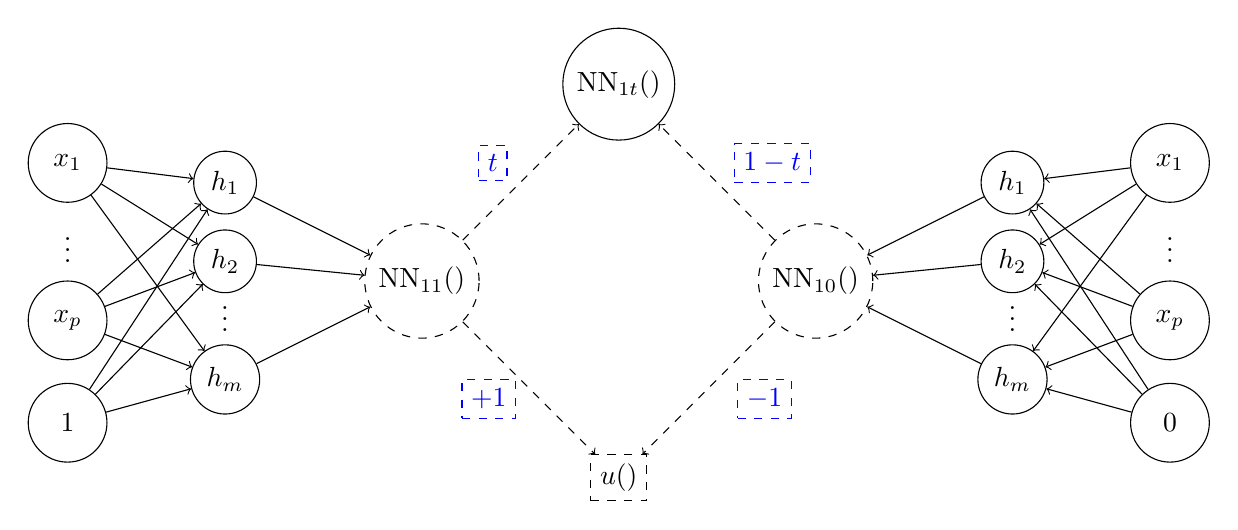
\begin{tikzpicture}
    
    
    \tikzset{dist/.style={path picture= {
    \begin{scope}[x=1pt,y=10pt]
      \draw plot[domain=-6:6] (\x,{1/(1 + exp(-\x))-0.5});
    \end{scope}
    }}}
    \tikzstyle{sigmoid}=[draw,fill=gray!20,circle,minimum size=20pt,inner sep=0pt,dist]
    
    
    % INPUT LAYER
    % T=1
    %\draw[red,thick,dashed] (-1,1) circle (3mm);
    \node(x11) at (-3,1) [circle, draw, minimum size=1cm] {$x_1$};
    \node at (-3,0) {$\vdots$};
    %\draw[red,thick,dashed] (-1,-1) circle (3mm);
    \node(x1p) at (-3,-1) [circle, draw, minimum size=1cm] {$x_p$};
    %\draw[blue,thick,dashed] (-1,-2) circle (3mm);
    \node(t1) at (-3,-2.3) [circle, draw, minimum size=1cm] {$1$};

    
    % T=0
    %\draw[red,thick,dashed] (9,1) circle (3mm);
    \node(x21) at (11,1) [circle, draw, minimum size=1cm] {$x_1$};
    \node at (11,0) {$\vdots$};
    %\draw[red,thick,dashed] (9,-1) circle (3mm);
    \node(x2p) at (11,-1) [circle, draw, minimum size=1cm] {$x_p$};
    %\draw[blue,thick,dashed] (9,-2) circle (3mm);
    \node(t0) at (11,-2.3) [circle, draw, minimum size=1cm] {$0$};
  
    % HIDDEN LAYER
    % T=1
    %\draw[black,thick,dashed] (1,0.75) circle (3mm);
    \node(h11) at (-1,0.75) [circle, draw] {$h_1$};
    %\draw[black,thick,dashed] (1,0) circle (3mm);
    \node(h12) at (-1,-0.25) [circle, draw] {$h_2$};
    \node at (-1,-0.875) {$\vdots$};
    %\draw[black,thick,dashed] (1,-1.75) circle (3mm);
    \node(h1m) at (-1,-1.75) [circle, draw] {$h_m$};
     % T=0
    %\draw[black,thick,dashed] (7,0.75) circle (3mm);
    \node(h21) at (9,0.75) [circle, draw] {$h_1$};
    %\draw[black,thick,dashed] (7,0) circle (3mm);
    \node(h22) at (9,-0.25) [circle, draw] {$h_2$};
    \node at (9,-0.875) {$\vdots$};
    %\draw[black,thick,dashed] (7,-1.75) circle (3mm);
    \node(h2m) at (9,-1.75) [circle, draw] {$h_m$};
    
    % CENTER OF THE FIGURE
    % T=t
    %\draw[red,thick,dashed] (4,-0.5) circle (3mm);
    %\node(true_t) at (4,-0.5) {$t$};
    % CONDITIONAL MEANS 
    %\draw[black,thick,dashed]  (2.5, -0.5) circle (7mm);
    \node (p1)[] at (1.5, -0.5) [circle, draw, dashed] {$\mathrm{NN}_{11}(\x)$};
    %\node (p1)[sigmoid] at (2.5, -0.5) {};
    %\node (p0)[sigmoid] at (5.5, -0.5) {};
    %\draw[black,thick,dashed]  (5.5, -0.5) circle (7mm);
    \node (p0)[] at (6.5, -0.5) [circle, draw, dashed] {$\mathrm{NN}_{10}(\x)$};
    
    % WEIGHTS
    %1st layer T=1
    \draw[->] (x11) -- (h11) node [midway,above] {};
    \draw[->] (x1p) -- (h11) node [midway,above] {};
    \draw[->] (t1) -- (h11) node [midway,above] {};
    
    \draw[->] (x11) -- (h12) node [midway,above] {};
    \draw[->] (x1p) -- (h12) node [midway,above] {};
    \draw[->] (t1) -- (h12) node [midway,above] {};
    
    \draw[->] (x11) -- (h1m) node [midway,above] {};
    \draw[->] (x1p) -- (h1m) node [midway,above] {};
    \draw[->] (t1) -- (h1m) node [midway,above] {};
    
    %1st layer T=0
    \draw[->] (x21) -- (h21) node [midway,above] {};
    \draw[->] (x2p) -- (h21) node [midway,above] {};
    \draw[->] (t0) -- (h21) node [midway,above] {};
    
    \draw[->] (x21) -- (h22) node [midway,above] {};
    \draw[->] (x2p) -- (h22) node [midway,above] {};
    \draw[->] (t0) -- (h22) node [midway,above] {};
    
    \draw[->] (x21) -- (h2m) node [midway,above] {};
    \draw[->] (x2p) -- (h2m) node [midway,above] {};
    \draw[->] (t0) -- (h2m) node [midway,above] {};
    
    %2nd layer
    \draw[->] (h11) -- (p1) node [midway,above] {};
    \draw[->] (h12) -- (p1) node [midway,below] {};
    \draw[->] (h1m) -- (p1) node [midway,below] {};
    
    \draw[->] (h21) -- (p0) node [midway,above] {};
    \draw[->] (h22) -- (p0) node [midway,below] {};
    \draw[->] (h2m) -- (p0) node [midway,below] {};
    
    
    %OUTPUT
    %\draw[black,thick] (4,-3) circle (6mm);
    \node(uplift) at (4,-3) [rectangle, draw, dashed] {$u(\x)$};
    
    %\draw[black,thick] (4,2) circle (7mm);
    \node(mean) at (4,2) [circle, draw] {$\mathrm{NN}_{1t}(\x)$};
    
    %OUTPUT CONNEXIONS
     %\draw[->, dashed] (true_t) -- (mean);
    \draw[->, dashed] (p1) -- (mean); %node [midway,above] {$t$};
    \node at (2.4,1) [rectangle, draw, blue, dashed] {$t$};
    \draw[->, dashed] (p0) -- (mean); %node [midway,above] {$(1-t)$};
    \node at (5.95,1) [rectangle, draw, blue, dashed] {$1-t$};
    
    \draw[->, dashed] (p1) -- (uplift); %node [midway,above] {$+1$};
    \node at (2.35,-2) [rectangle, draw, blue, dashed] {$+1$};
    \draw[->, dashed] (p0) -- (uplift); %node [midway,above] {$-1$};
    \node at (5.85,-2) [rectangle, draw, blue, dashed] {$-1$};
    
    
    \end{tikzpicture}}
    \caption{A twin neural model for uplift. The inputs contain the covariates vector $\x$ and, for the left sub-component, the treatment variable fixed to $1$. The treatment variable is fixed to $0$ for the right sub-component. The sub-components output the predicted conditional means for treated ($\mathrm{NN}_{11}(\x)$) and for control ($\mathrm{NN}_{10}(\x)$). The difference gives direct prediction of $u(\x)$. At the same time, the predicted conditional mean $\mathrm{NN}_{1t}(\x)$ is based on the actual received treatment for each individual $t \in \{0,1\}$, i.e., $\mathrm{NN}_{1t}(\x) = t \mathrm{NN}_{11}(\x) + (1-t) \mathrm{NN}_{10}(\x)$.}
    \label{fig:nite}
\end{figure}
